\documentclass[12pt,a4paper,UTF8]{ctexart}
	%10pt:正文字体为12pt,缺省为10pt;各层级字体大小会根据正文字体自动调整
	%a4paper:纸张大小a4;
	%UTF8:中文要求
\usepackage{geometry}%用于设置上下左右页边距
	\geometry{left=2.5cm,right=2.5cm,top=3.2cm,bottom=2.8cm}
\usepackage{xeCJK,amsmath,paralist,enumerate,booktabs,multirow,graphicx,subfig,setspace,listings,lastpage,hyperref,setspace}
	%xeCJK:中文字体(如楷体,作者和机构需要用到)的设置
	%amsmath:数学公式
	%paralist,enumerate:自定义项目符号
	%booktabs:三线图,论文常用的表格风格
	%multirow:复杂表格
	%graphicx,float: 插入图片
	%subfig:并排排版图片、竖向排版图片
	%setspace:设置行间距等功能
	\setlength{\parindent}{2em}%正文首行缩进两个汉字
	%listings:用于排版各种代码;比如matlab的代码
	\lstset{language=Matlab}%matlab代码
	%lastpage:获取总页数;
	%hyperref:超链接,和lastpage搭配.
\usepackage{fancyhdr}
	%fancyhdr:一个很强大的宏包,用于自定义设计页面风格并命名以供调用。
	\pagestyle{fancy}
	\rhead{实验B11 圆孔衍射实验}
	\lhead{基础物理实验\uppercase\expandafter{\romannumeral2}会议摘要}
	\cfoot{Page \thepage/\pageref{LastPage}}  %当前页\总页数
		%分别是右页眉、左页眉、中页脚、右页脚
	\renewcommand{\headrulewidth}{0.4pt}
	\renewcommand{\theenumi}{(\arabic{enumi})}
	\setlength\headheight{15pt}
\usepackage{longtable}

\begin{document}

%%begin-------------------标题与信息-----------------------%%

%%标题
\begin{center}
\LARGE\textbf{实验B11 圆孔衍射实验}
\end{center}



\subsection*{【数据处理】}
\subsubsection*{1.夫琅禾费衍射}
实验现象:亮度不断变亮,其中心一直为亮斑,没有亮暗变化。

原理解释: 由公式可知,艾里斑半径的衍射角度与圆孔半径成反比,所以当小孔半径减小
时,直径 D减小,艾里斑尺寸越来越小,且从激光器发出的光为平行光,在中央明纹处始
终相干叠加增强,因此不会有明暗变化。

\begin{table}[htbp]
	\centering
	  \caption{夫琅禾费衍射实验数据}
	\resizebox{\textwidth}{16mm}{ %第一个大括号为宽度,第二个大括号为高度(60mm)可随机设置,调整到适合该表格的大小为止
	  \begin{tabular}{cccc}
	  \toprule
	  孔径D/mm & 主极大位置/mm & 第一暗纹位置/mm & 艾里斑半径R/mm \\
	  \midrule
	  0.15 &19.786&12.287&7.50\\
	  0.3 & 14.12 & 10.96 &3.16\\
	  0.5 & 9.00 & 6.67 & 2.33 \\
	  \bottomrule
	  \end{tabular}}%注意这里还有一个半括号
	\label{tab:1}%
  \end{table}
本实验光探头离圆孔距离足够远,故使用远场近似,艾里斑半径有理论值:
\begin{equation*}
	R=1.22\frac{\lambda}{D}l
\end{equation*}
其中$\lambda=632.8nm$,$l=67.8cm$,代入得不同孔径下的理论艾里斑半径。

  \begin{table}[htbp]
	\centering
	  \caption{艾里斑半径实验值与理论值比较}
	\resizebox{\textwidth}{14mm}{ %第一个大括号为宽度,第二个大括号为高度(60mm)可随机设置,调整到适合该表格的大小为止
	  \begin{tabular}{ccccc}
	  \toprule
	  孔径D/mm &孔径倒数/$mm^{-1}$& 理论半径$R_0$/mm & 实验半径R/mm & 相对误差/\%\\
	  \midrule
	  0.15 &6.67&6.98&7.50&7.4\\
	  0.3  & 3.33 & 3.49&3.16&9.4\\
	  0.5  & 2 & 2.09& 2.33& 11.5\\
	  \bottomrule
	  \end{tabular}}%注意这里还有一个半括号
	\label{tab:2}%
  \end{table}

  \begin{figure}[htbp]
	\centering
	\includegraphics[width=0.8\textwidth]{img//plot.jpeg}
	\label{fig:1}
\end{figure}

由相关性检验得到t值为7.5526,自由度为1对应的p值为0.0838,Pearson相关系数为0.9913481,理论与实际相关性较好。

实验过程分析误差原因有:
\begin{enumerate}
	\item 距离较近时光斑直径过小不便于观测,肉眼判断中心亮斑和暗斑判断不准确
	\item 使用刻度尺测量精度不够,出现误差,且我们组所用刻度尺有断裂现象,增大误差
	\item 最亮和最暗的位置无法准确判断,在某个区间中为亮斑,在另一个区间中为暗斑,肉眼无法分析亮度大小
\end{enumerate}

\subsubsection*{2.菲涅尔圆孔衍射}
实验现象:初始时光屏距离圆孔板较近,光斑很小,中央亮度很高。
随着距离的不断增大,衍射光斑也逐渐增大,光斑中心衍射条纹逐渐清晰,中心光斑随着光屏和圆孔板的距离增大
不断交替出现亮-暗-亮-暗的变化。

原理解释:由半波带理论,波前可以分割为一系列环形带,在白屏上某点的合成振幅则为各
个半波带振幅的叠加。改变观察屏和圆孔板的距离时候,半波带的数目会发生变化,当半波
带数 k为奇数时,屏中央为亮斑;k为偶数时,屏中央为暗斑,所以移动过程中会出现亮-暗-亮-暗的变化。

\begin{table}[htbp]
	\centering
	  \caption{菲涅尔衍射实验数据}
	\resizebox{0.6\textwidth}{12mm}{ %第一个大括号为宽度,第二个大括号为高度(60mm)可随机设置,调整到适合该表格的大小为止
	  \begin{tabular}{ccc}
	  \toprule
	  孔径D/mm & 亮纹位置/cm & 暗纹位置/cm  \\
	  \midrule
	  1.5 &81.2&61.3\\
	  1 & 67.9 & 41.5 \\
	  \bottomrule
	  \end{tabular}}%注意这里还有一个半括号
	\label{tab:3}%
  \end{table}
  *圆孔位置为22.1cm.
  
  通过半波带的计算验证测量的合理性:

  完整的菲涅尔波带数目k 与单透镜和圆孔之间的距离R ,圆孔的半径$\rho $ 、光的波长$\lambda$ 以及
  圆孔和观察屏距离b之间的关系为:
  \begin{align*}
	  k&=\frac{\rho^2(R+b)}{\lambda b R}
	   =\frac{\rho^2}{\lambda}\left(\frac{1}{b}+\frac{1}{R}\right)\\
  \end{align*}

将所得实验结果与理论值比较得:
\begin{table}[htbp]
	\centering
	  \caption{菲涅尔衍射实验值与理论值比较}
	\resizebox{\textwidth}{16mm}{ %第一个大括号为宽度,第二个大括号为高度(60mm)可随机设置,调整到适合该表格的大小为止
	  \begin{tabular}{cccccc}
	  \toprule
	  孔径D/mm&圆孔到光探头距离/cm &中心点& 半波带理论数目 & 奇偶 & 相对误差/\%\\
	  \midrule
	 1.5 &亮&59.1&40.537&奇&1.31\\
	  1.5  & 暗 & 39.2&28.913&偶&3.26\\
	  1 & 亮 & 45.8& 18.792& 奇&1.09\\
	  1&暗 &19.4&23.488&偶&2.13\\
	  \bottomrule
	  \end{tabular}}%注意这里还有一个半括号
	\label{tab:4}%
  \end{table}


  实验过程分析误差原因有:
\begin{enumerate}
	\item 衍射小孔并不是规整的圆孔导致艾里斑并不是标准的圆形,引起测量误差
	\item 艾里斑与周围的暗条纹并不是严格地泾渭分明,所以测量所得的艾里斑直径比真实值偏差
\end{enumerate}


\subsection*{【思考题】}
\subsubsection*{1.列举可以获得衍射光斑光强分布的方法,并简述其原理。}
(1)一种基于CCD相机的多角度电弧光采集方法

电弧等离子体作为一种自发光观测对象,本方法不需要旋转电弧或移动相机的情况下,利用反射镜在180$^{\circ}$范围内角度下发出的电弧光,
最后窄带滤光片选取所需波段的光进入到相机中,
最终不同角度下的电弧窄带图像呈现在相机感光元件的不同位置上,完成多角度下的特定谱线光强分布采集。
其中,中继镜头对电弧进行二次对焦,一定程度上缩短或延长了工业相机的对焦距离,使相机在相同焦距下对不同光程的光都可以清晰成像,且电弧像的大小相同。

(2)数码相机测量相对光强分布

采用数码相机直接拍摄艾里斑,记多数码相机与艾里斑之间的距离,然后在相同距离下用数码相机拍摄毫米尺的像将艾里究和毫米尺两张图片进行比对,可以较精确地获得艾里斑直径的数值。
采用 Photoshop 或 MatLab 软件编程,根据拍摄图片的灰度还可以获得圆孔衍射光斑相对光强分布的定量数据。

(3)采用光纤光功率计测量衍射光斑的相对光强分布
采用的光纤光功率计的纤芯直径只有62.5um,可测量空间指定点的光强,将功率计输入光纤安装在一维(z方向)平移底座上,光纤指向与光轴平行,并与艾里斑的水平直径处在同一高度。平移输入光纤,记录光功率计读数与水平位置的数值。

\subsubsection*{2.菲涅尔圆孔衍射和夫琅禾费衍射图像的图样有何异同?}
在菲涅尔衍射区,随着观察屏距离的变化,仅考察轴上衍射图样,会出现明暗交替的情况。
在夫琅禾费衍射区,随着观察屏距离的变化,衍射图样会在轴上不会出现明暗交替的情况,衍射斑的大小会变化,但形状一直不变,而强度与观察角度有关。

\subsubsection*{3.在满足远场条件下,狭缝前后也可以不用透镜而获得夫琅禾费衍射图样。请简述远场条件。}
远场条件为$\frac{D^2}{l\lambda}\ll 1$,其中D为孔径,l为光屏到圆孔距离,$\lambda$为光源波长。

\subsubsection*{4.采用数值计算的方法画出多种圆孔直径、多种圆孔距离下的艾里斑图样。}
R语言作出光强热图:
\begin{figure}[htbp]
	\centering
	\subfloat[孔径=1.5mm,圆孔距离=115cm]{\label{fig:8.2}
	\includegraphics[width=0.4\textwidth]{img//plot115.jpeg}
	}
	\subfloat[孔径=0.15mm,圆孔距离=89.5cm]{\label{fig:8.3}
	\includegraphics[width=0.4\textwidth]{img//plot2.jpeg}
	}

	\subfloat[孔径=1.5mm,圆孔距离=40cm]{\label{fig:8.4}
	\includegraphics[width=0.4\textwidth]{img//plot3.jpeg}
	}
	\subfloat[孔径=1mm,圆孔距离=90cm]{\label{fig:8.5}
	\includegraphics[width=0.4\textwidth]{img//Rplot.jpeg}
	}
	\caption{艾里斑}
	\label{fig:2}
\end{figure}



将各项基本光学参数按照上述的数据进行设定,并用Matlab的PDE tool进行处理得到如下图样。

1.当圆孔直径为0.15mm时,观察屛和圆孔距离为
\begin{figure}[htbp]
	\centering
	\includegraphics[width=0.3\textwidth]{img//0.251.jpg}
	\includegraphics[width=0.3\textwidth]{img//0.252.jpg}
	\includegraphics[width=0.3\textwidth]{img//0.253.jpg}
	\caption{0.25m}
\end{figure}

\begin{figure}[htbp]
	\centering
	\includegraphics[width=0.3\textwidth]{img//0.51.jpg}
	\includegraphics[width=0.3\textwidth]{img//0.52.jpg}
	\includegraphics[width=0.3\textwidth]{img//0.53.jpg}
	\caption{0.5m}
\end{figure}

\begin{figure}[htbp]
	\centering
	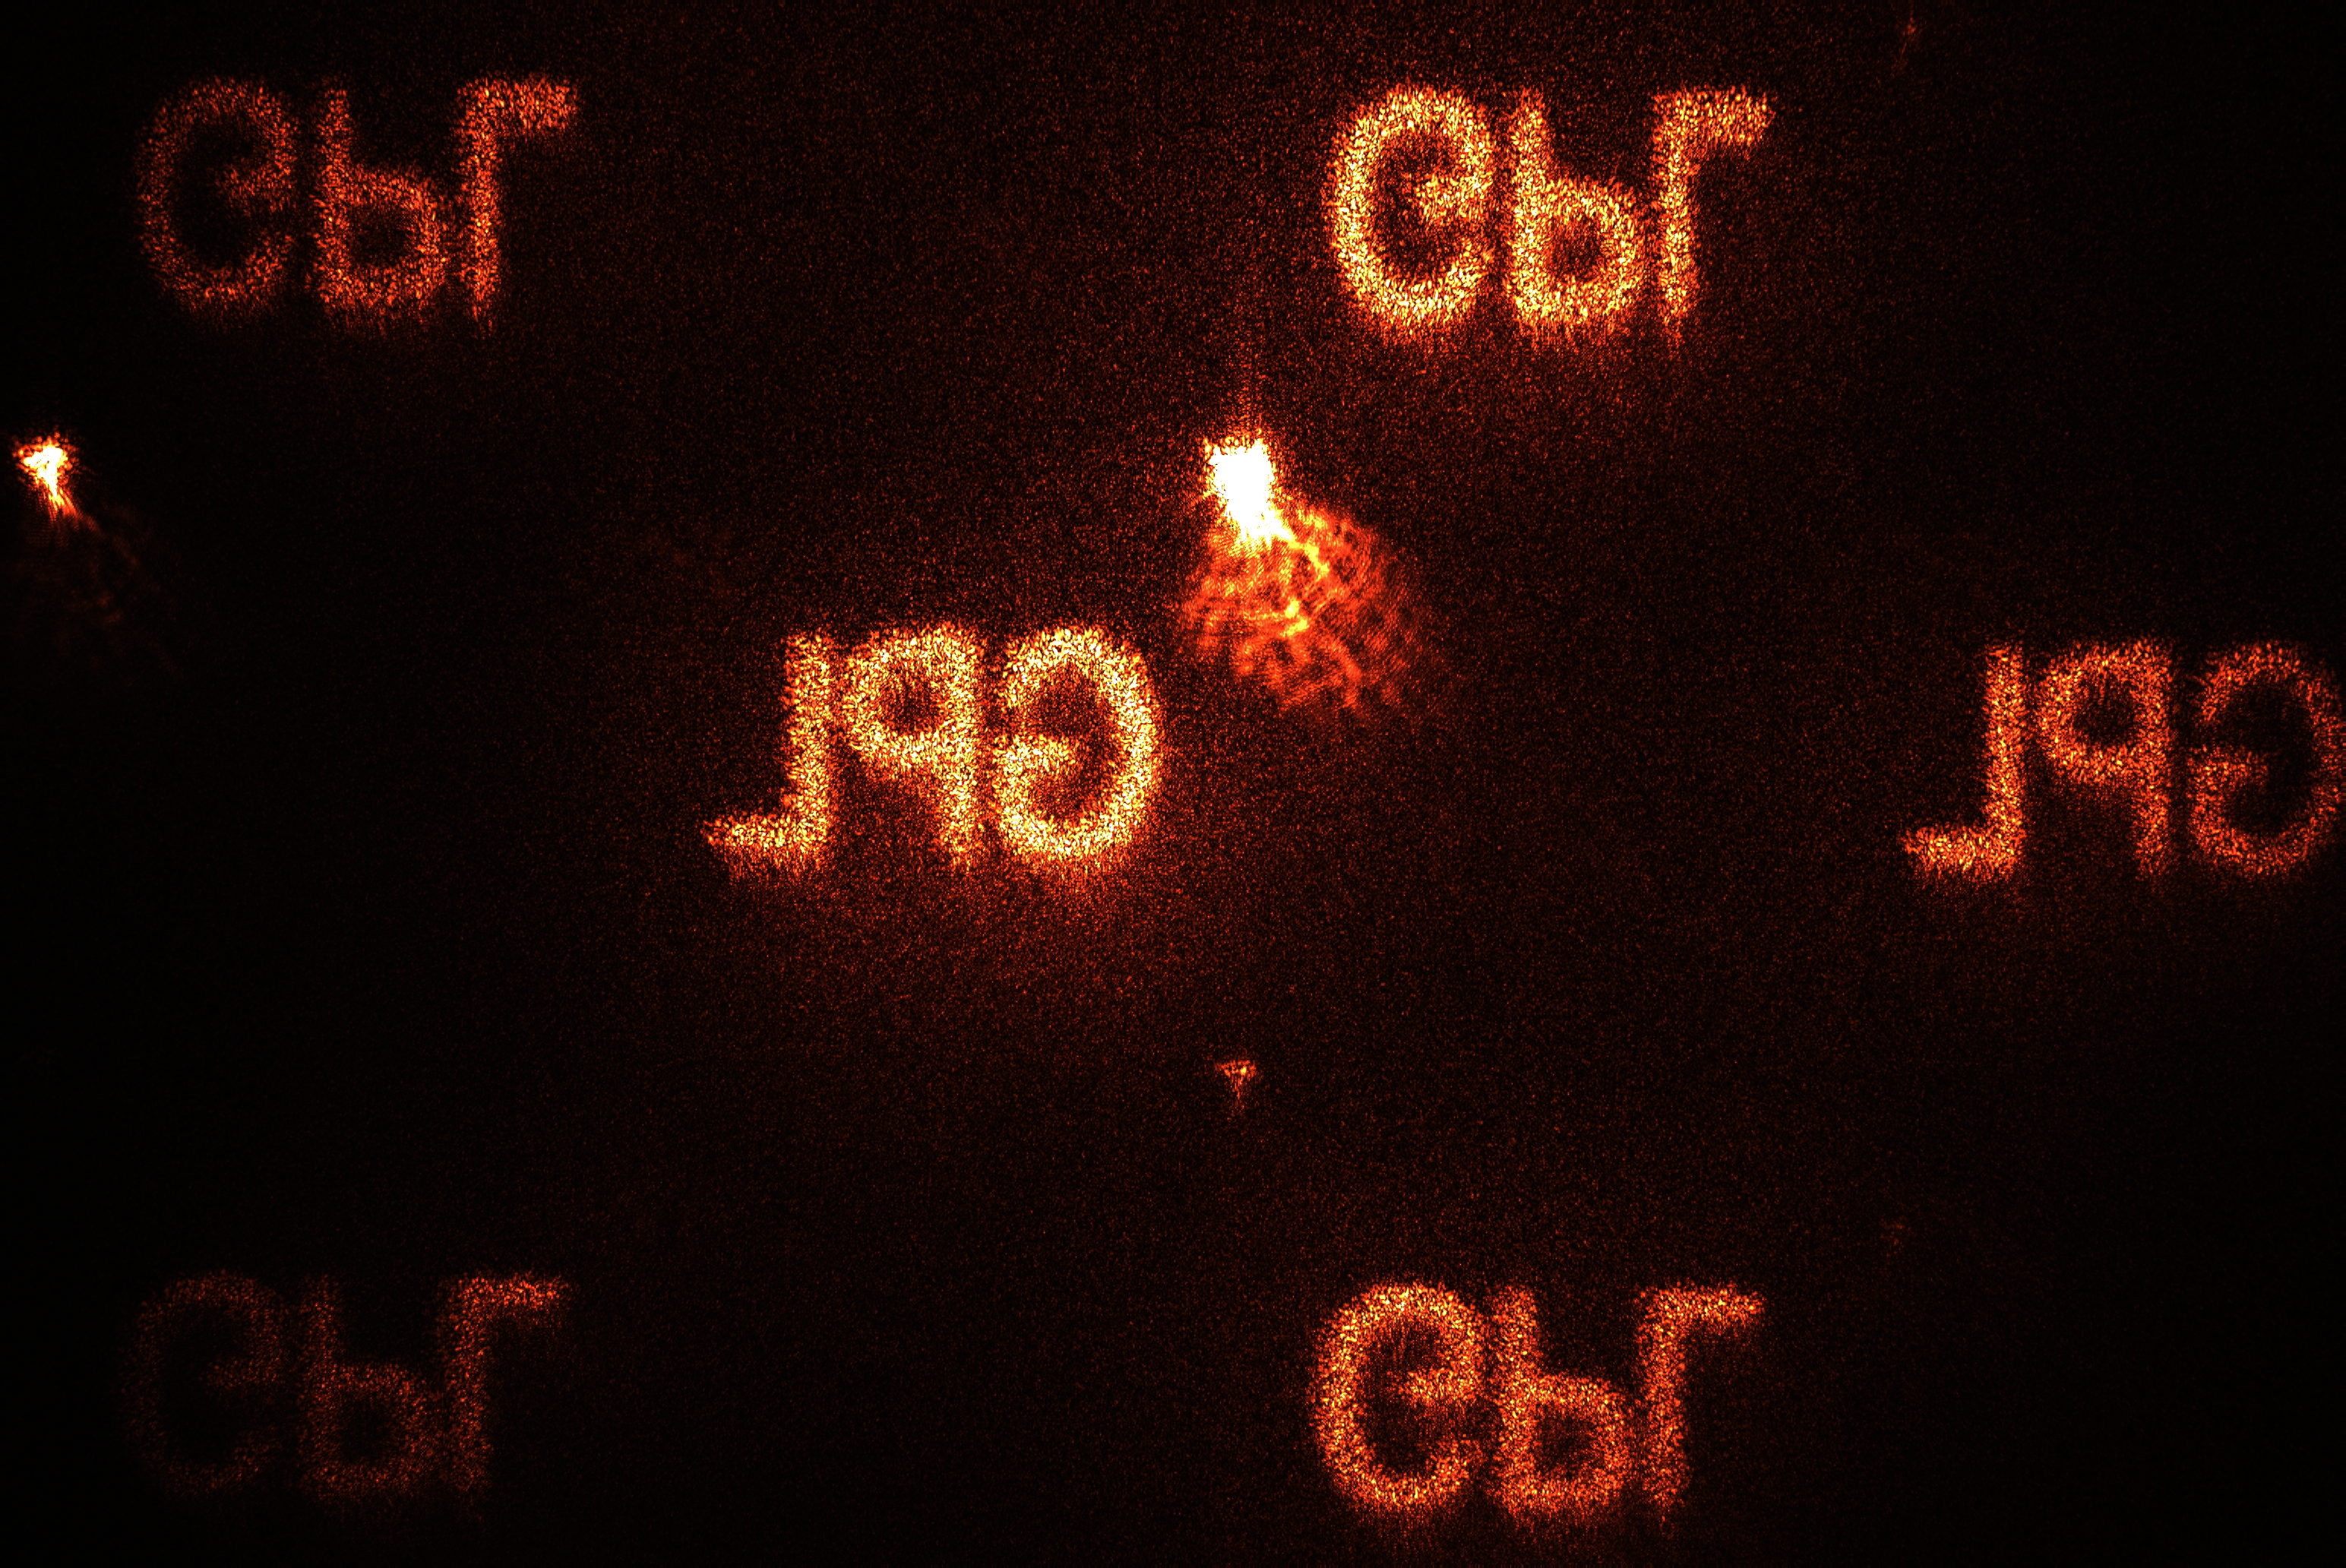
\includegraphics[width=0.3\textwidth]{img//1.1.jpg}
	\includegraphics[width=0.3\textwidth]{img//1.2.jpg}
	\includegraphics[width=0.3\textwidth]{img//1.3.jpg}
	\caption{1m}
\end{figure}
\newpage
2.当圆孔直径为0.3mm时,观察屛和圆孔距离为
\begin{figure}[htbp]
	\centering
	\includegraphics[width=0.3\textwidth]{img//0.257.jpg}
	\includegraphics[width=0.3\textwidth]{img//0.258.jpg}
	\includegraphics[width=0.3\textwidth]{img//0.259.jpg}
	\caption{0.25m}
\end{figure}

\begin{figure}[htbp]
	\centering
	\includegraphics[width=0.3\textwidth]{img//0.57.jpg}
	\includegraphics[width=0.3\textwidth]{img//0.58.jpg}
	\includegraphics[width=0.3\textwidth]{img//0.59.jpg}
	\caption{0.5m}
\end{figure}

\begin{figure}[htbp]
	\centering
	\includegraphics[width=0.3\textwidth]{img//1.7.jpg}
	\includegraphics[width=0.3\textwidth]{img//1.8.jpg}
	\includegraphics[width=0.3\textwidth]{img//1.9.jpg}
	\caption{1m}
\end{figure}
\newpage
3.当圆孔直径为0.7mm时,观察屛和圆孔距离为
\begin{figure}[htbp]
	\centering
	\includegraphics[width=0.3\textwidth]{img//0.254.jpg}
	\includegraphics[width=0.3\textwidth]{img//0.255.jpg}
	\includegraphics[width=0.3\textwidth]{img//0.256.jpg}
	\caption{0.25m}
\end{figure}

\begin{figure}[htbp]
	\centering
	\includegraphics[width=0.3\textwidth]{img//0.54.jpg}
	\includegraphics[width=0.3\textwidth]{img//0.55.jpg}
	\includegraphics[width=0.3\textwidth]{img//0.56.jpg}
	\caption{0.5m}
\end{figure}

\begin{figure}[htbp]
	\centering
	\includegraphics[width=0.3\textwidth]{img//1.4.jpg}
	\includegraphics[width=0.3\textwidth]{img//1.5.jpg}
	\includegraphics[width=0.3\textwidth]{img//1.6.jpg}
	\caption{1m}
\end{figure}


\end{document}